% Author:   Sarah Lawrence
%           sarahy.lawrence@gmail.com 

\documentclass[a4paper,11pt]{article}

\usepackage[T1]{fontenc}
\usepackage[utf8]{inputenc}
\usepackage{graphicx}
\usepackage{xcolor}
\usepackage{graphicx}
\usepackage{subcaption}


\renewcommand\familydefault{\sfdefault}
\usepackage{tgheros}
\usepackage{amsmath,amssymb,amsthm,textcomp}
\usepackage{enumerate}
\usepackage{multicol}
\usepackage{tikz}
\usepackage{courier}


\usepackage{geometry}
\geometry{left=25mm,right=25mm,%
bindingoffset=0mm, top=20mm,bottom=20mm}


\linespread{1.3}

\newcommand{\linia}{\rule{\linewidth}{0.5pt}}

% Titles
\makeatletter
\renewcommand{\maketitle}{
\begin{center}
\vspace{2ex}
{\huge \textsc{\@title}}
\vspace{1ex}
\\
\linia\\
\@author \hfill \@date
\vspace{4ex}
\end{center}
}
\makeatother
%%%

% custom footers and headers
\usepackage{fancyhdr}
\pagestyle{fancy}
\lhead{}
\chead{}
\rhead{Bulldog Game}
\lfoot{Bulldog Improvements}
\cfoot{}
\rfoot{Page \thepage}
\renewcommand{\headrulewidth}{0pt}
\renewcommand{\footrulewidth}{0pt}
%

% code listing settings
\usepackage{listings}
\usepackage{color}

\definecolor{dkgreen}{rgb}{0,0.6,0}
\definecolor{gray}{rgb}{0.5,0.5,0.5}
\definecolor{mauve}{rgb}{0.58,0,0.82}

\lstset{frame=tb,
  language=Java,
  aboveskip=3mm,
  belowskip=3mm,
  showstringspaces=false,
  columns=flexible,
  basicstyle={\small\ttfamily},
  numbers=none,
  numberstyle=\tiny\color{gray},
  keywordstyle=\color{blue},
  commentstyle=\color{dkgreen},
  stringstyle=\color{mauve},
  breaklines=true,
  breakatwhitespace=true,
  tabsize=3
}



% dice set up 
\usepackage{pifont}
\DeclareFontFamily{U}{dice3d}{}
\DeclareFontShape{U}{dice3d}{m}{n}{<-> s*[4] dice3d}{}

%%%----------%%%----------%%%----------%%%----------%%%

\begin{document}

\title{Random Singleness}

\author{Sarah Lawrence, University of Southern Maine}

\date{04/09/2025}

\maketitle

\section*{Description}
\hrule
\vspace{13pt} % Adjusts space after the line
The purpose of this assignment is to gain experience with the Singleton design pattern and to develop a framework in which one can test methods that use randomness as part of their computations. Additionally, it provides an opportunity to assess, at least in part, the ability to implement design patterns effectively.


\section*{Build a First Singleton}
\hrule
\vspace{10pt} % Adjusts space after the line
The task was to use AI (ChatGPT 3.5) to rewrite that class as a singleton. Then compare the code created by that tool to the style of singleton shown in the lecture. Preparation for the task involved creating a referee class. This was to contain the program responsible for the logic that runs a game of Bulldog. Then convert it to singleton using AI. Building and comparing the AI and lecture singletons can be seen below.

\vspace{5pt} % Adjusts space after the line
\subsection*{AI Singleton Results:}
Building the Singleton took over 2 minutes and 10 seconds with AI. This includes bug testing. Overall, it was successful on the second prompt. There were a couple of changes that the AI made to the original work. The prompts and changes are as follows.\\
Prompt:
\hrule
\vspace{4pt} % Adjusts space after the line
\begin{quote}
\textbf{Human:} Rewrite that class as a Singleton (referee class code) \\
\textbf{ChatGPT:}To rewrite the Referee class as a Singleton, you'll need to ensure that only one instance of the class exists throughout the application. (code) \\\\
Some of the old referee class:
\begin{lstlisting}
public class Referee {
    private PlayerList players;
    private int currentPlayerIndex;
    
    public Referee(PlayerList players) {
        this.players = players;
        this.currentPlayerIndex = 0;
    }

    public Player getCurrentPlayer() {
        return players.getPlayers().get(currentPlayerIndex);
    }

\end{lstlisting} (This code keeps going) \\\\
Some of the new  referee class: \begin{lstlisting}
public class Referee {
    private static Referee instance;  // Singleton instance
    private PlayerList players;
    private int currentPlayerIndex;

    // Private constructor to prevent instantiation
    private Referee(PlayerList players) {
        this.players = players;
        this.currentPlayerIndex = 0;
    }

    // Public method to provide access to the instance
    public static Referee getInstance(PlayerList players) {
        if (instance == null) {
            instance = new Referee(players);
        }
        return instance;
    }

    public Player getCurrentPlayer() {
        return players.getPlayers().get(currentPlayerIndex);
    }
\end{lstlisting}
(This code keeps going)
\end{quote}
the constructor was made private and created a getInstance() method. \\
The only thing that didn't work was in the GameGUI the line
\begin{lstlisting}
referee = new Referee(playerList);
\end{lstlisting} It was changed to \begin{lstlisting}
referee = Referee.getInstance(playerList);
\end{lstlisting} Then the code ran successfully.


\subsection*{Lecture Singleton}
Building this singleton was not required. This singleton is from the Gang of Four book or lecture L03.26 slide 10, created by David Levine. What it looks like can be seen below. \\\\
Lecture singleton:
\begin{lstlisting}
public class MySingleton {
    private static MySingleton instance = null;  
    private int myVariable;

    private MySingleton() {
        //Private constructor to prevent iteration from outside the class 
        myVariable = 0;
    }

    public static MySingleton getInstance() {
        //Lazy initalization the instance is created when the getinstance() method is first called
        if(instance == null){
            instance = new MySingleton();
        }
        return instance;
    }

    public int getMyVariable() {
        return myVariable;
    }

    public void setMyVariable(int newValue) {
        myVariable = newValue;
    }
}
\end{lstlisting}

\subsection*{Comparison}
They both succeeded in implementing the Singleton Pattern. This is because both classes restrict instantiation using a private static instance and a private constructor. They both also create the instance only when getInstance() is first called. They did have differences. Their purpose, parameters, and methods were a bit different. These differences can be seen better in the table below. \\\\\\ 

\begin{table}[h!]
\centering
\begin{tabular}{|p{3cm}|p{5cm}|p{5cm}|}
\hline
\textbf{Aspect} & \textbf{Referee} & \textbf{MySingleton} \\
\hline
Purpose & Manages turn-based game using a PlayerList. & A generic singleton with a variable myVariable. \\
\hline
Constructor & Takes a PlayerList parameter. & Takes no parameters. \\
\hline
\text{getInstance()} Method & Requires a PlayerList argument on the first call. & Takes no arguments. \\
\hline
Use Case & Built for coordinating a game (turns, players, game end). & Generic example could be adapted to anything. \\
\hline
\end{tabular}
\label{tab:singleton-comparison}
\end{table}

\section*{Change Dice class}
\hrule
\vspace{10pt} % Adjusts space after the line
I prompted the AI to create the object of the Random class in the Dice class as a Singleton. When completed, it should be able to have Dice of different sizes. For example, 6 and 2 would be the ones that would be used. While ensuring they all share a Singleton Random object.\\
Prompt:
\hrule
\vspace{4pt} % Adjusts space after the line
\begin{quote}
\textbf{Human:} Change things so that the object of the Random class in your Dice class is a Singleton. When you are done, you will be able to have Dice of different sizes (6 and 2 would be the ones you would use - the former in all cases, and the latter for RandomPlayer) but all of those would share a Singleton Random object. (Dice code)\\
\textbf{ChatGPT:} (new dice class code) 
\end{quote}
It took in total 1 minutes and 13 seconds to complete and bug test. The old and new code can be seen below.\\\\
Old Dice class:
\begin{lstlisting}
import java.util.Random;

public class Dice {
    private Random random;

    public Dice() {
        random = new Random();
    }

    public int roll() {
        return random.nextInt(6) + 1;
    }
}
\end{lstlisting} 
New Dice class: \begin{lstlisting}
import java.util.Random;

public class Dice {
    private static final Random random = new Random();
    private final int dice_sides;

    public Dice(int dice_sides) {
        this.dice_sides = dice_sides;
    }

    public int roll() {
        return random.nextInt(dice_sides) + 1; 
    }
}
\end{lstlisting}
What's changed was a couple of things. One is that private Random random; is now private static final Random random = new Random();. Making it only one instance of random. Another is the addition of a new variable for the dice sides called dice\_sides.  This new variable was added to the method dice. Allowing the dice to change size. Here is a test that helped show that the dice can change size using the singleton random object. \\\\
DiceTest class: \begin{lstlisting}
public class DiceTest {
    public static void main(String[] args) {
        Dice d6 = new Dice(6);
        Dice d2 = new Dice(2);

        System.out.println("Rolling d6 (6-sided) 10 times:");
        for (int i = 0; i < 10; i++) {
            System.out.print(d6.roll() + " ");
        }

        System.out.println("\nRolling d2 (2-sided) 10 times:");
        for (int i = 0; i < 10; i++) {
            System.out.print(d2.roll() + " ");
        }
    }
}
\end{lstlisting}
Results from terminal:
\begin{figure}[h] 
    \centering
    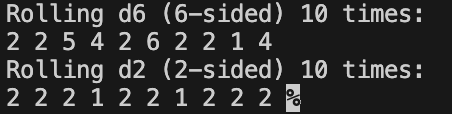
\includegraphics[width=0.45\textwidth]{DiceTest.png}
    \label{fig:first}
\end{figure}\\
As can be seen the 6 sided dice displays random numbers ranging from 1-6. While the two sided dice only has random numbers ranging from 1-2.
\section*{Create an abstract RandomDice superclass}
\hrule
\vspace{10pt} % Adjusts space after the line
My IDE didn't allow me to extract a superclass from a class. So I made the AI do it. It took me 1 minute and 47 seconds to make and bug test. My superclass kept track of the number of sides of the Dice and have an abstract roll() method. The Random object stayed with the Dice class.\\\\
Reminder of the old Dice class:
\begin{lstlisting}
import java.util.Random;

public class Dice {
    private static final Random random = new Random();
    private final int dice_sides;

    public Dice(int dice_sides) {
        this.dice_sides = dice_sides;
    }

    public int roll() {
        return random.nextInt(dice_sides) + 1; 
    }
}
\end{lstlisting} 
New Dice class: \begin{lstlisting}
import java.util.Random;

public class Dice extends RandomDice {
    private static final Random random = new Random(); // Singleton Random instance

    public Dice(int sides) {
        super(sides); // Call constructor of RandomDice
    }

    @Override
    public int roll() {
        return random.nextInt(sides) + 1; // Random number between 1 and sides
    }
}
\end{lstlisting}
New abstract RandomDice superclass: \begin{lstlisting}
public abstract class RandomDice {
    protected final int sides;

    public RandomDice(int sides) {
        this.sides = sides;
    }

    public abstract int roll();
}
\end{lstlisting}

\section*{JUnit Testing}
\subsection*{Create a FakeRandom subclass of RandomDice}
The FakeRandom implemented the roll method. In this class, it's not pretending to be random. I prompted the AI to perform the task here were the prompts.\\\\
Prompts:
\hrule
\vspace{4pt} % Adjusts space after the line
\begin{quote}
\textbf{Human:} in Junit "Create a FakeRandom subclass of RandomDice. FakeRandom should implement the roll method (Dice and RandomDice code)\\
\textbf{ChatGPT:} Great! You’re working with a dice-rolling abstraction where RandomDice is the base class, Dice uses real randomness....
\end{quote}
This prompt produced two FakeRandom classes one that was simple and only tested one roll. The other was a little more complex but allowed to test multiple rolls. The two are provided below. \\\\
One roll FakeRandom class:
\begin{lstlisting}
public class FakeRandom extends RandomDice {
    private final int fixedRoll;

    public FakeRandom(int sides, int fixedRoll) {
        super(sides);
        this.fixedRoll = fixedRoll;
    }

    @Override
    public int roll() {
        return fixedRoll;
    }
}
\end{lstlisting}
Multi roll FakeRandom class:
\begin{lstlisting}
public class FakeRandom extends RandomDice {
    private final int[] sequence;
    private int index;

    public FakeRandom(int sides, int... sequence) {
        super(sides);
        this.sequence = sequence;
        this.index = 0;
    }

    @Override
    public int roll() {
        int value = sequence[index % sequence.length];
        index++;
        return value;
    }
}
\end{lstlisting}
I used the second code FakeRandom class cause I wanted to test multiple rolls. Overall, This process took seconds.\\
After creating the code I wanted to test it. I wanted to see if AI could create a Junit test to make sure the code was working properly. The AI created the following.  
\begin{lstlisting}
import static org.junit.Assert.*;
import org.junit.Test;

public class FakeRandomTest {

    @Test
    public void testFixedRoll() {
        RandomDice dice = new FakeRandom(6, 4);
        assertEquals(4, dice.roll());
        assertEquals(4, dice.roll()); // Should always return 4
    }

    @Test
    public void testSequenceRolls() {
        RandomDice dice = new FakeRandom(6, 2, 5, 3);
        assertEquals(2, dice.roll());
        assertEquals(5, dice.roll());
        assertEquals(3, dice.roll());
        assertEquals(2, dice.roll()); // Loops back
    }
}
\end{lstlisting}
 In the testFixedRoll test, the dice is initialized to always return the fixed value 4. The test checks that multiple calls to roll() consistently return 4. In the testSequenceRolls method, the dice are initialized with a sequence of values (2, 5, 3). The test checks that roll() returns these values in order. It loops back to the start once the sequence ends. These tests ensure correct behavior from FakeRandom, making it useful to check for errors. After performing the tests on the code it passed. 

\subsection*{Create a SevenPlayer class}
SevenPlayer was designed just like FifteenPlayer but stops at 7 rather than 15. My FifteenPlayer  I found out wasn't working properly so it was fixed and changed to SevenPlayer. This took 12 minutes with AI to fix. Changing it from 15 to 7 took me only seconds. Here is some of the code below. \\\\
SevenPlayer class code:
\begin{lstlisting}
rollButton.addActionListener(new ActionListener() {
            @Override
            public void actionPerformed(ActionEvent e) {
                if (!isCurrentPlayer()) return;
                
                // Initialize Dice object
                Dice dice = new Dice(6);
                int roll = 0;
                turn_total = getTurnTotal();
    
                // Continue rolling until 7 is rolled
                while (turn_total <= 7) {
                    roll = dice.roll();

                    if (roll == 6) {
                        rollResultLabel.setText("Roll: " + roll);
                        turnTotalLabel.setText("Turn Total: 0");
                        setTurnTotal(0);
\end{lstlisting} (This code keeps going)

\subsection*{Create a FakeRandom test class}
I created a JUnit test case with sufficient tests to verify that your SevenPlayer class works properly. I don't have a panel with a green bar so to show that it works I will provide Visual Studio's method of showing the tests pass. \\
First, let's talk about the tests the AI created. I didn't prompt it to create certain tests I just asked it to make tests that would check if SevenPlayerTest is working properly. With this prompt, the AI created three tests. The first test was testStopsAtSix, this test checks if rolling a 6 resets the turn total 0. It also makes sure the total is 0 since getting a 6 shouldn't add anything to the total. This test can be seen below.\\\\
SevenPlayerTest class testStopsAtSix test:
\begin{lstlisting}
 @Test
    public void testStopsAtSix() throws Exception {
        FakeRandom fakeDice = new FakeRandom(6, 6); // rolls a 6 immediately
        setupPlayer(fakeDice);

        SwingUtilities.invokeAndWait(() -> rollButton.doClick());

        assertEquals("Roll: 6", rollResultLabel.getText());
        assertEquals("Turn Total: 0", turnTotalLabel.getText());
        assertEquals("Total: 0", scoreLabel.getText());
        assertFalse(rollButton.isEnabled());
    }
\end{lstlisting} (This keeps going)\\
The second test is named testRollsUntilOverSeven. It mimics rolling a sequence of 3 and 2 repeatedly until the total exceeds 7. For example, it rolls a 3, then a 2, adds them together, and checks whether the sum is greater than 7. If not, it continues adding another 3, and so on. Once the total exceeds 7, the test verifies that the turn total is updated correctly.
\begin{lstlisting}
 @Test
    public void testRollsUntilOverSeven() throws Exception {
        FakeRandom fakeDice = new FakeRandom(6, 3, 2); // sum = 8
        setupPlayer(fakeDice);

        SwingUtilities.invokeAndWait(() -> rollButton.doClick());

        assertEquals("Turn Total: 8", turnTotalLabel.getText());
        assertFalse(rollButton.isEnabled());
    }
\end{lstlisting}
The final test the AI created was called testRollsAndThenSix. This test had one roll then a roll with a 6. This was to test if the turn total would be 0 despite rolling a 2 earlier. 
\begin{lstlisting}
 @Test
    public void testRollsAndThenSix() throws Exception {
        FakeRandom fakeDice = new FakeRandom(6, 2, 6); // should reset to 0 at 6
        setupPlayer(fakeDice);

        SwingUtilities.invokeAndWait(() -> rollButton.doClick());

        assertEquals("Roll: 6", rollResultLabel.getText());
        assertEquals("Turn Total: 0", turnTotalLabel.getText());
        assertFalse(rollButton.isEnabled());
    }
\end{lstlisting}
In the end, my code ended up passing the AI tests. Since I don't have a completion bar to show that this is true instead I'll show the check marks. A green check mark means the test passed, while a red circle with a dot indicates a failure. In the figure below, all the tests are listed on the left side, and the code for each individual test is shown on the right.\\\\  
Results:
\begin{figure}[h] 
    \centering
    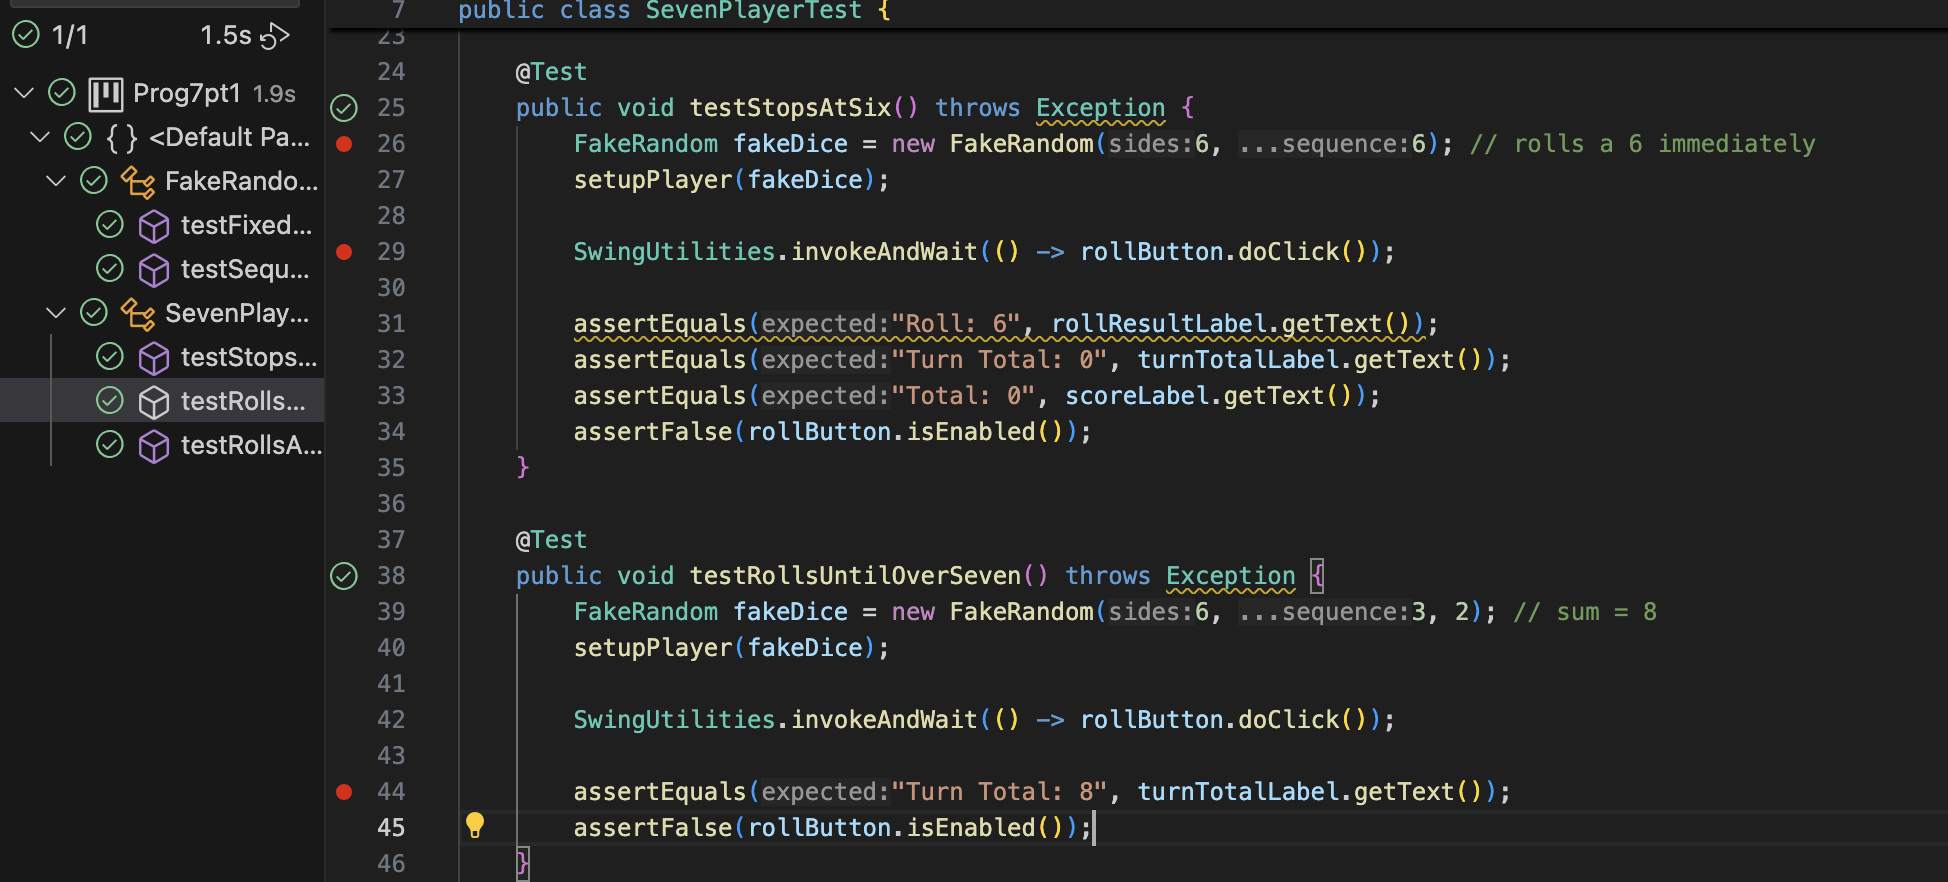
\includegraphics[width=0.80\textwidth]{JunitTest.png}
    \label{fig:first}
\end{figure}\\
The only change I would make is creating more tests. One such test would be making sure the total is updated correctly. I would do this; however, I moved this feature outside of the Seven-player class due to repetitive code. Since this is moved this is outside of the scope of this task. But this will be experimented on in the future.

\section*{Javadoc}
\hrule
\vspace{10pt} 
Putting the code into Javadoc style took over 5 minutes and 6 seconds with AI. The headers "Written by Sarah Lawrence, with the assistance of ChatGBT 3.5." were done by hand. \\
The process was to do one class at a time and ask the model to format the code in Javadoc. The model had no problems completing the tasks. Here is some example code showing the successes of the model.\\\\
Main class Example:
\begin{lstlisting}
/**
 * A player implementation for the Bulldog game that keeps rolling the dice
 * until their turn total exceeds 7 or they roll a 6 (which ends their turn with 0 points).
 * This class uses Swing components for interaction and display.
 */
public class SevenPlayer extends Player {
    /** Button to initiate a dice roll */
    private JButton rollButton;

    /** Label to display the result of a dice roll */
    private JLabel scoreLabel;

    /** Label to display the score result of a turn */
    private JLabel rollResultLabel;

    /** Label to display the cumulative total of the current turn */
    private JLabel turnTotalLabel;
\end{lstlisting} (This keeps going)\\
I did this because in another experiment I tried asking the model to repeat the same step of changing the code to Javadoc. But I did it without specifying the step each time. When I did this the model had problems repeating the task. I then did another experiment where I used this method and it worked so I tried it again. I can confirm this method is far more effective than the first. 

\section*{Conclusion}
Altogether, ChatGBT did well in implementing all the steps. The AI didn't have trouble at all with these tasks. This could be due to the fact that it was done in parts and not all together or it just does very well with tasks like these. The only one that took the longest was Create a FakeRandom test class. This was due to user error as I struggled to set up and figure out how to use Junit in Visual Studios. Overall I would say the AI was successful at completing these tasks. 
\end{document}
